\section{Testes com utilizadores}

Em Julho de 2007 foram efectuados testes de usabilidade
na cidade de Glasgow, na Esc�cia, no �mbito do programa IMPROVE, em que o ImmiView se insere.

Participaram 10 utilizadores, estudantes de arquitectura e arquitectos.
Os mesmos foram distribu�dos em grupos de 2, realizando cada um um conjunto de tarefas em separado
e uma tarefa colaborativa, estando um deles munido dos marcadores.

%Dada a origem dos diferentes utilizadores (7 escoceses, 2 ingleses e 1 espanhol), verificou-se dificuldade em alguns deles em emitir comandos de voz correctamente reconhecidos pelo sistema.

% O arranque das ac��es com gestos necessitou de algumas tentativas. Em particular, o utilizador n�o marcado foi aconselhado a afastar-se durante o tracking.

%, tendo inviabilizado a tarefa de voo para um utilizador ap�s 3 tentativas falhadas.
%Em indiv�duos altos n�o houve qualquer problema%de captura de movimentos
%, o que leva a supor que os problemas ocorridos derivaram de oclus�es.

\begin{figure}[ht]
	\centering
	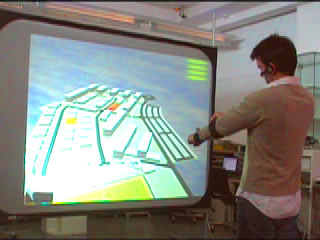
\includegraphics[width=.75\linewidth]{don.png}
	\vspace{-4mm}
	\caption{utilizador em modo voo}
	\label{fig:don}
\end{figure}

%\subsection{An�lise}

%Os utilizadores estranharam por vezes a utiliza��o dos comandos \textbf{begin} e \textbf{stop}.
%As alternativas \textbf{begin} / \textbf{end} ou \textbf{start} / \textbf{stop} seriam as mais l�gicas.
%No entanto as mesmas haviam sido testadas aquando dos primeiros testes de voz, tendo-se ent�o conclu�do que
%\textbf{start} / \textbf{stop} eram confundidos entre si pelo motor e que \textbf{end} originava falsos positivos.
%
%Foi sugerida a altera��o de \textbf{stop x} para simplesmente \textbf{stop}.
%Um utilizador em apuros na interac��o n�o consegue por vezes recordar o contexto em que est�,
%de modo a invocar o stop adequado.

